\chapter{Business Plan}

\section{Organizzazione Complessiva del Business Plan}

Il presente Business Plan ha l'obiettivo di valutare la sostenibilità economica e finanziaria di \textit{Tuning Ledger}, la piattaforma per la gestione del \textit{Digital Modified Vehicle Passport} (DMVP), il registro distribuito dedicato alla certificazione e alla tracciabilit\`a delle modifiche eseguite nel settore dell'automotive tuning.

Si assume che il progetto venga realizzato da una societ\`a di sviluppo software gi\`a operativa sul mercato, e non da una \textit{start-up}, impiegando esclusivamente personale interno. L'analisi finanziaria si sviluppa su un orizzonte temporale di \textbf{sei anni}, coerentemente con la pianificazione definita nel Project Plan (Capitolo~6):

\begin{itemize}
    \item \textbf{Fase 1 (Anno 0)}: progettazione, sviluppo e \textit{deployment} della piattaforma (durata 1 anno).
    \item \textbf{Fase 2 (Anni 1-5)}: promozione, commercializzazione, erogazione dei servizi di assistenza e manutenzione evolutiva (durata 5 anni).
\end{itemize}

Per la stima dei costi del personale si assume la quota standard di \textbf{1.752 ore lavorative} per un Anno/Persona (A/P), equivalenti a 219 giornate lavorative da 8 ore. Di seguito vengono analizzate le componenti di costo impiegate in entrambe le fasi.

\subsection{Costi del Personale}

Le figure professionali coinvolte nel progetto sono quelle individuate nel Project Plan. Per ciascun profilo viene esplicitata la classificazione contrattuale in conformit\`a con i livelli stabiliti dal Contratto Collettivo Nazionale dei Metalmeccanici attualmente in vigore:

\begin{itemize}
    \item \textbf{Project Manager (PM)}: livello Quadro (ex 8\textdegree{} livello), con retribuzione lorda mensile di 2.493,21 \euro{} e superminimo di 1.000,00 \euro{}.
    \item \textbf{Software Architect (SA)}: livello B3 (ex 7\textdegree{} livello), con retribuzione lorda mensile di 2.336,00 \euro{} e superminimo di 500,00 \euro{}.
    \item \textbf{Full Stack Developer (FSD)}: livello B2 (ex 6\textdegree{} livello), con retribuzione lorda mensile di 2.092,45 \euro{} e superminimo di 200,00 \euro{}.
    \item \textbf{Full Stack Developer Junior (FSDJ)}: livello B1 (ex 5\textdegree{} Super), con retribuzione lorda mensile di 1.950,39 \euro{}, senza superminimo.
\end{itemize}

La Retribuzione Annua Lorda (RAL) si ottiene moltiplicando la retribuzione mensile globale, comprensiva di eventuale superminimo, per tredici mensilit\`a. Al fine di determinare il costo aziendale effettivo, alla RAL sono stati addizionati i seguenti elementi, con gli esiti riepilogati in Tabella~\ref{tab:costo-personale}:

\begin{itemize}
    \item \textbf{Trattamento di Fine Rapporto (TFR)}: calcolato mediante la formula RAL / 13,5, equivalente a poco meno di una mensilit\`a aggiuntiva.
    \item \textbf{Oneri previdenziali a carico dell'azienda}: determinati sulla base di un'aliquota contributiva complessiva stimata al 36\% della RAL, ripartita in due terzi a carico del datore di lavoro (\textbf{24\%}) e un terzo a carico del lavoratore (12\%).
\end{itemize}

\begin{table}[H]
\centering
\begin{tabular}{lrrrr}
\hline
\textbf{Profilo} & \textbf{RAL} & \textbf{TFR} & \textbf{Oneri azienda} & \textbf{Costo annuo} \\
\hline
PM   & 45.411,73 & 3.363,83 & 10.898,82 & 59.674,38 \\
SA   & 36.868,00 & 2.730,96 &  8.848,32 & 48.447,28 \\
FSD  & 29.801,85 & 2.207,54 &  7.152,44 & 39.161,84 \\
FSDJ & 25.355,07 & 1.878,15 &  6.085,22 & 33.318,44 \\
\hline
\end{tabular}
\caption{Costo lordo aziendale annuo per figura professionale (valori in \euro)}
\label{tab:costo-personale}
\end{table}

\subsection{Spese Generali}

Nell'assetto economico aziendale, le spese generali raggruppano tutti gli oneri necessari a garantire la continuit\`a e il corretto funzionamento delle attivit\`a operative, incluse le fasi di sviluppo software. Pur non essendo direttamente imputabili alla realizzazione del singolo servizio, tali costi risultano essenziali per il supporto dell'intera struttura d'impresa. Tra le principali voci si distinguono:

\begin{itemize}
    \item \textbf{Affitti e locazioni}: canoni relativi agli spazi aziendali destinati a uffici e aree operative.
    \item \textbf{Spese amministrative e gestionali}: costi legati sia al personale interno deputato al management, sia a servizi professionali esterni quali lo studio commercialista per la contabilit\`a e il consulente del lavoro per l'elaborazione dei cedolini.
    \item \textbf{Utenze e servizi infrastrutturali}: oneri per energia elettrica, riscaldamento, connettivit\`a e servizi di base necessari al mantenimento dell'infrastruttura aziendale.
\end{itemize}

Al fine di semplificare la valutazione dell'incidenza di tali flussi di spesa sul budget complessivo, l'analisi adotta una stima forfettaria pari al \textbf{20\% del costo totale del personale}.

\subsection{Costi per il Cloud Computing}

Nel contesto di un'azienda di sviluppo software, i costi legati alle risorse di calcolo e di memorizzazione non rientrano tra le spese generali, in quanto direttamente imputabili alle attivit\`a tecnico-operative. L'adozione di soluzioni \textit{cloud} consente di ottimizzare l'efficienza finanziaria tramite modelli di \textit{pricing} basati sul consumo effettivo (\textit{pay-per-use}), azzerando gli investimenti iniziali in hardware e i relativi costi di manutenzione.

Si assume pertanto che i servizi computazionali e di storage siano erogati interamente in cloud, ivi compresi i nodi della rete \textit{permissioned} e il database \textit{off-chain} destinato alla documentazione tecnica associata al DMVP. Il costo associato a ciascuna unit\`a $X$ del gruppo di lavoro \`e determinato mediante la seguente equazione:

\begin{equation}
    \text{Costo Totale} = (C_M \times 12) + (C_O \times N_O)
\end{equation}

dove $C_M$ \`e il costo fisso mensile del servizio cloud, $C_O$ il costo orario delle risorse di calcolo e $N_O$ il numero annuo di ore di utilizzo previsto per ciascun ruolo. Per la simulazione d'impatto sono stati adottati i valori $C_M = 20$ \euro{} e $C_O = 2$ \euro{}, con il seguente monte ore annuo: 600 ore per il Project Manager, 1.100 ore per il Software Architect e 1.300 ore per ciascun Full Stack Developer, senior e junior. Ne derivano i costi annui per persona riportati in Tabella~\ref{tab:cloud}.

\begin{table}[H]
\centering
\begin{tabular}{lrr}
\hline
\textbf{Profilo} & \textbf{Ore annue} & \textbf{Costo annuo} \\
\hline
PM   &   600 & 1.440,00 \\
SA   & 1.100 & 2.440,00 \\
FSD  & 1.300 & 2.840,00 \\
FSDJ & 1.300 & 2.840,00 \\
\hline
\end{tabular}
\caption{Costo annuo del cloud computing per unit\`a di personale (valori in \euro)}
\label{tab:cloud}
\end{table}

\subsection{Costi per Oneri Finanziari e Tassazione}

Gli oneri finanziari rappresentano i costi derivanti dagli interessi passivi sui capitali di terzi, necessari a coprire il fabbisogno di liquidit\`a del progetto nelle fasi antecedenti la generazione dei flussi di ricavo attesi. L'accesso alle linee di credito non costituisce tuttavia un processo automatico: gli istituti di credito subordinano l'erogazione dei finanziamenti a una rigorosa valutazione del merito creditizio dell'azienda, richiedendo idonee garanzie patrimoniali e un'approfondita analisi della sostenibilit\`a economico-finanziaria dell'iniziativa. Per la pianificazione del presente progetto, l'incidenza degli oneri finanziari \`e stata stimata prudenzialmente applicando un tasso d'interesse pari al \textbf{12\% annuo} sull'ammontare del capitale finanziato.

Oltre agli interessi passivi, la pianificazione finanziaria deve integrare la componente fiscale, rappresentata dall'Imposta sul Reddito delle Societ\`a (\textbf{IRES}, con aliquota del 24\%) e dall'Imposta Regionale sulle Attivit\`a Produttive (\textbf{IRAP}, con aliquota del 4,82\% per la regione Calabria). L'incidenza di tali imposte risulta determinante ai fini di una corretta valutazione strategica, poich\'e incide direttamente sulla redditivit\`a netta del progetto e, di conseguenza, sulla sostenibilit\`a finanziaria complessiva dell'iniziativa nel lungo periodo.

\section{Analisi dei Costi della Fase 1}

La quantificazione degli oneri relativi all'Anno Zero integra le differenti componenti economiche indispensabili all'avvio e al \textit{deployment} del progetto. La stima analitica, riepilogata in Tabella~\ref{tab:costi-fase1}, si articola attraverso le seguenti voci di spesa:

\begin{itemize}
    \item \textbf{Costo del personale}: determinato dal prodotto tra l'impegno complessivo espresso in Anni-Persona e il costo annuo lordo aziendale di ciascuna figura professionale allocata, secondo la distribuzione definita nel Project Plan.
    \item \textbf{Spese generali}: pari al 20\% del costo del personale, secondo la stima forfettaria illustrata in precedenza.
    \item \textbf{Costi di cloud computing}: calcolati in conformit\`a al modello descritto nella sezione precedente, parametrizzati in funzione della quota di impegno dei singoli profili.
    \item \textbf{Consulenze esterne}: relative all'ingaggio di esperti di dominio esterni al nucleo aziendale, con competenze verticali nel settore dell'omologazione e delle modifiche veicolari, stimate in 20.000,00 \euro{}.
\end{itemize}

\begin{table}[H]
\centering
\begin{tabular}{lr}
\hline
\textbf{Fase 1} & \textbf{Costo} \\
\hline
P: Costo del personale            & 456.350,04 \\
SG: Spese generali (20\% di P)    &  91.270,01 \\
Costi di cloud computing          &  31.570,00 \\
Consulenze esterne                &  20.000,00 \\
\hline
\textbf{C: COSTO TOTALE}          & \textbf{599.190,05} \\
O: Oneri finanziari su C          &  71.902,81 \\
\textbf{CO: COSTO CON ONERI}      & \textbf{671.092,86} \\
OF2: Oneri finanziari su CO       &  80.531,14 \\
Rata di ammortamento              & 134.218,57 \\
\hline
\end{tabular}
\caption{Analisi dei costi della Fase 1 (valori in \euro)}
\label{tab:costi-fase1}
\end{table}

\section{Analisi dei Costi e dei Ricavi della Fase 2}

La Fase 2, estesa su un orizzonte temporale di cinque anni, raggruppa l'insieme degli oneri operativi necessari al mantenimento e alla commercializzazione della piattaforma (Tabella~\ref{tab:costi-fase2}). Alle voci gi\`a illustrate per la Fase 1, ricalcolate sull'organico ridotto previsto per l'esercizio, si aggiungono:

\begin{itemize}
    \item \textbf{Consulenze esterne}: pianificate secondo un \textit{trend} decrescente, a fronte della progressiva autonomia tecnica acquisita dal team interno. L'onere si attesta a 15.000,00 \euro{} nel primo anno per poi ridursi a 10.000,00 \euro{} nelle annualit\`a successive.
    \item \textbf{Ammortamento dei costi di sviluppo}: quota di ripartizione pluriennale dell'investimento iniziale sostenuto nell'Anno Zero, pari a 134.218,57 \euro{} per ciascuno dei cinque anni di esercizio.
\end{itemize}

Nell'analisi dei costi complessivi assume rilevanza critica la valutazione degli oneri finanziari, che si suddividono in due macro-categorie:

\begin{enumerate}
    \item \textbf{Oneri finanziari associati al finanziamento iniziale}: relativi al capitale preso a prestito per coprire i costi di sviluppo della piattaforma nell'Anno Zero. Il valore di riferimento \`e l'onere OF2, pari a 80.531,14 \euro{}, che si contrae linearmente di 16.106,23 \euro{} ogni anno coerentemente con un piano di ammortamento quinquennale.
    \item \textbf{Oneri finanziari derivanti da disavanzi operativi}: riconducibili ai flussi di cassa negativi che si manifestano qualora le spese di gestione superino i ricavi di periodo. Si ipotizza che tali squilibri vengano colmati mediante linee di credito aggiuntive, gravate dal medesimo tasso nominale annuo del 12\%.
\end{enumerate}

I ricavi aziendali, riportati in Tabella~\ref{tab:ricavi-fase2}, sono stati stimati sulla base delle seguenti assunzioni strategiche, coerenti con i flussi individuati nel Business Model Canvas e con l'individuazione dell'Intermediario quale cliente primario della piattaforma:

\begin{itemize}
    \item \textbf{Canone di abbonamento flat}: l'accesso alla piattaforma prevede una quota fissa annua pari a 30.000,00 \euro{} per intermediario, considerata costante per l'intero quinquennio di proiezione.
    \item \textbf{Pricing delle verticalizzazioni}: il corrispettivo unitario per ciascuna verticalizzazione \`e fissato a 5.000,00 \euro{} per il primo anno, si riduce a 4.000,00 \euro{} nel secondo e si stabilizza a 3.000,00 \euro{} per il restante triennio.
    \item \textbf{Crescita del portafoglio clienti}: si prevede un incremento graduale del numero di intermediari abbonati, da 10 unit\`a nel primo anno a 40 nel quinto. Si stima che ciascun intermediario richieda in media 2 verticalizzazioni nel corso del primo anno e 3 verticalizzazioni annue dal secondo al quinto.
\end{itemize}

Si osservi che il Business Model Canvas prevede, tra i flussi di ricavo, anche un addebito proporzionale al volume di DMVP registrati e certificati sulla piattaforma. Tale voce non \`e stata inclusa nella presente proiezione per ragioni prudenziali, in quanto subordinata a volumi di adozione difficilmente stimabili nella fase di avvio; essa costituisce pertanto un potenziale margine di ricavo ulteriore rispetto a quanto qui rappresentato.

\begin{table}[H]
\centering
\small
\makebox[\textwidth][c]{%
\begin{tabular}{lrrrrrr}
\hline
\textbf{Ricavi Fase 2} & \textbf{Anno 1} & \textbf{Anno 2} & \textbf{Anno 3} & \textbf{Anno 4} & \textbf{Anno 5} & \textbf{Totale} \\
\hline
Numero intermediari        &      10 &      15 &      20 &      25 &        40 &       110 \\
Totale abbonamenti         & 300.000 & 450.000 & 600.000 & 750.000 & 1.200.000 & 3.300.000 \\
Numero verticalizzazioni   &      20 &      45 &      60 &      75 &       120 &       320 \\
Totale verticalizzazioni   & 100.000 & 180.000 & 180.000 & 225.000 &   360.000 & 1.045.000 \\
\hline
\textbf{RICAVO TOTALE}     & \textbf{400.000} & \textbf{630.000} & \textbf{780.000} & \textbf{975.000} & \textbf{1.560.000} & \textbf{4.345.000} \\
\hline
\end{tabular}}
\caption{Ricavi della Fase 2 (valori in \euro)}
\label{tab:ricavi-fase2}
\end{table}

\begin{table}[H]
\centering
\small
\makebox[\textwidth][c]{%
\begin{tabular}{lrrrrrr}
\hline
\textbf{Costi Fase 2} & \textbf{Anno 1} & \textbf{Anno 2} & \textbf{Anno 3} & \textbf{Anno 4} & \textbf{Anno 5} & \textbf{Totale} \\
\hline
P: Personale             & 265.658 & 265.658 & 265.658 & 265.658 & 265.658 & 1.328.291 \\
SG: Spese generali       &  53.132 &  53.132 &  53.132 &  53.132 &  53.132 &   265.658 \\
Cloud per esercizio      &  18.980 &  18.980 &  18.980 &  18.980 &  18.980 &    94.900 \\
Consulenze esterne       &  15.000 &  10.000 &  10.000 &  10.000 &  10.000 &    55.000 \\
Ammortamento piattaforma & 134.219 & 134.219 & 134.219 & 134.219 & 134.219 &   671.093 \\
\hline
\textbf{B: COSTO TOTALE} & \textbf{486.988} & \textbf{481.988} & \textbf{481.988} & \textbf{481.988} & \textbf{481.988} & \textbf{2.414.942} \\
C: Oneri fin.\ piattaforma &  80.531 &  64.425 &  48.319 &  32.212 &  16.106 &   241.593 \\
D: Oneri su disavanzo      &       0 &  20.102 &  12.484 &       0 &       0 &    32.587 \\
\hline
\textbf{BC: COSTI TOTALI}  & \textbf{567.520} & \textbf{566.516} & \textbf{542.791} & \textbf{514.201} & \textbf{498.095} & \textbf{2.689.122} \\
\hline
\end{tabular}}
\caption{Costi della Fase 2 (valori in \euro)}
\label{tab:costi-fase2}
\end{table}

Una volta calcolati i ricavi \`e possibile rappresentare l'analisi complessiva dei costi e dei ricavi dei primi cinque anni di attivit\`a della piattaforma, comprensiva dei costi associati agli eventuali disavanzi operativi e del carico fiscale di periodo (Tabella~\ref{tab:costi-ricavi}).

\begin{table}[H]
\centering
\small
\makebox[\textwidth][c]{%
\begin{tabular}{lrrrrr}
\hline
 & \textbf{Anno 1} & \textbf{Anno 2} & \textbf{Anno 3} & \textbf{Anno 4} & \textbf{Anno 5} \\
\hline
A -- RICAVI                  &  400.000 &  630.000 &  780.000 &  975.000 & 1.560.000 \\
BC -- COSTI TOTALI           &  567.520 &  566.516 &  542.791 &  514.201 &   498.095 \\
R1 -- Risultato lordo        & -167.520 &   63.484 &  237.209 &  460.799 & 1.061.905 \\
T1 -- IRES (24\% di R1)      &        0 &   15.236 &   56.930 &  110.592 &   254.857 \\
IR -- Imponibile IRAP        &   98.139 &  329.143 &  502.867 &  726.457 & 1.327.564 \\
T2 -- IRAP (4,82\% di IR)    &    4.730 &   15.865 &   24.238 &   35.015 &    63.989 \\
\hline
\textbf{R2 -- Risultato netto} & \textbf{-172.250} & \textbf{32.383} & \textbf{156.040} & \textbf{315.192} & \textbf{743.059} \\
\textbf{RC -- Risultato cumulato} & \textbf{-172.250} & \textbf{-139.867} & \textbf{16.174} & \textbf{331.366} & \textbf{1.074.425} \\
\hline
\end{tabular}}
\caption{Analisi costi-ricavi della Fase 2 (valori in \euro)}
\label{tab:costi-ricavi}
\end{table}

\section{Valutazione Complessiva del Business Plan}

\begin{figure}[H]
    \centering
    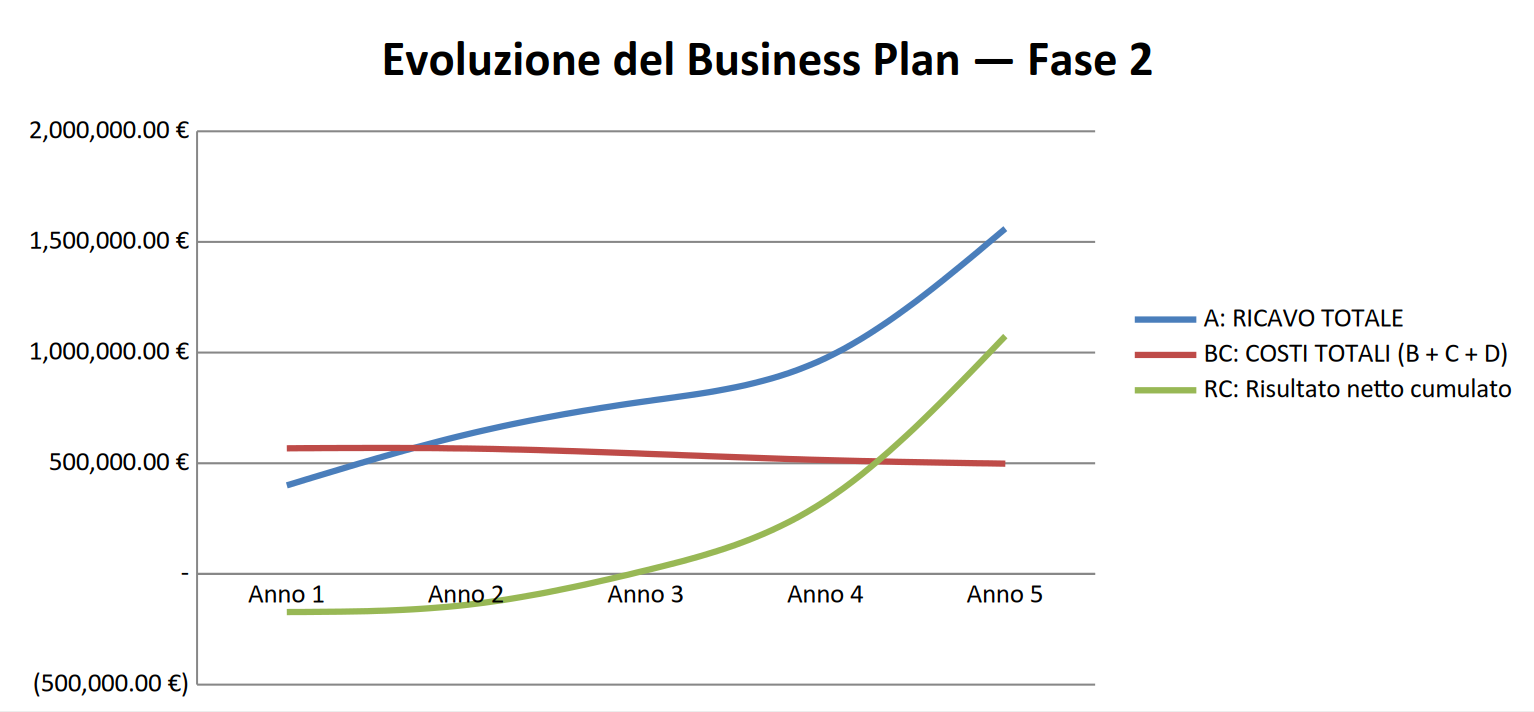
\includegraphics[width=\textwidth]{imgs/evoluzione.png}
    \caption{Evoluzione del Business Plan --- grafico di ricavi, costi e risultato netto cumulato nei cinque anni}
    \label{fig:evoluzione}
\end{figure}

Attraverso l'analisi dei dati previsionali \`e possibile determinare il \textbf{Break Even Point} (BEP). Il punto di pareggio individua il momento in cui il risultato netto cumulato dell'esercizio azzera l'investimento iniziale sostenuto nell'Anno~Zero: fino a quel momento l'iniziativa sta ancora recuperando il capitale impiegato, da quel momento in avanti inizia ad accumulare utile. Osservando la curva del \textit{Risultato Netto Cumulato} in Figura~\ref{fig:evoluzione}, si rileva che essa interseca l'asse dello zero in corrispondenza del \textbf{terzo anno} di esercizio, quando il risultato cumulato passa da $-139.867$ \euro{} a $+16.174$ \euro{}: da quel momento in avanti l'iniziativa economica inizia a generare un utile reale.

Un secondo indicatore fondamentale per valutare la sostenibilit\`a del progetto \`e il \textbf{ROI} (\textit{Return on Investment}), indice finanziario che misura la redditivit\`a del capitale investito esprimendo il guadagno generato per ogni euro allocato nella piattaforma:

\begin{equation}
    ROI = \frac{\text{Utile Netto}}{\text{Capitale Investito}} \times 100
\end{equation}

Coerentemente con la convenzione adottata, il \textbf{rendimento medio annuo} \`e ricavato dal
ROI sottraendo la quota del 100\% corrispondente alla restituzione del capitale investito e
ripartendo il residuo sui cinque anni di esercizio, in modo da esprimere il guadagno netto
prodotto mediamente in ciascuna annualit\`a per ogni euro allocato nella piattaforma.

\begin{table}[H]
\centering
\begin{tabular}{lr}
\hline
Risultato netto cumulato & 1.074.425,25 \\
Capitale investito       &   671.092,86 \\
\hline
\textbf{ROI in 5 anni}   & \textbf{160,10\%} \\
Rendimento annuo: (ROI $-$ 100\%) / 5 & 12,02\% \\
\hline
\end{tabular}
\caption{Indicatori di redditivit\`a del progetto}
\label{tab:roi}
\end{table}

I risultati ottenuti confermano la sostenibilit\`a economico-finanziaria dell'iniziativa (Tabella~\ref{tab:roi}). La piattaforma \`e in grado di assorbire l'investimento iniziale di 671.092,86 \euro{} e i costi ricorrenti di esercizio, raggiungendo il punto di pareggio nel corso del terzo anno di attivit\`a e generando, al termine del quinquennio, un risultato netto cumulato di circa 1,07 milioni di euro, con un rendimento medio annuo del 12,02\%.

\`E opportuno osservare che il pareggio viene raggiunto con un margine contenuto: il risultato cumulato del terzo anno si attesta a poco pi\`u di 16.000 \euro{}, valore che rende il conseguimento del BEP entro tale termine sensibile a scostamenti anche modesti nel ritmo di acquisizione dei clienti.

\`E opportuno inoltre osservare che il modello adottato si fonda su un'ipotesi di crescita graduale e prudente del portafoglio clienti e che non contabilizza alcuni dei flussi di ricavo previsti dal Business Model Canvas, quali l'addebito proporzionale al volume di DMVP registrati e il marketplace di servizi aggiuntivi. Il profilo di redditivit\`a rappresentato pu\`o pertanto essere considerato conservativo. Il principale fattore di rischio economico resta legato al ritmo di adesione degli intermediari alla piattaforma: un rallentamento nell'acquisizione dei primi clienti comporterebbe un incremento degli oneri su disavanzo operativo e un conseguente slittamento del Break Even Point, coerentemente con quanto evidenziato nell'analisi SWOT in merito alla necessit\`a di raggiungere una massa critica di attori nella filiera.